
% !TEX encoding = UTF-8 Unicode 
% !TEX root = FieldGuide.tex

\Sec{Gamma-Exponential Distribution}
\label{sec:GammaExp}
\phantomsection
\addcontentsline{toc}{subsection}{~~~~~~~~~~~~Gamma-exponential} 

The {\bf gamma-exponential} (log-gamma, generalized Gompertz, generalized Gompertz-Verhulst type I, Coale-McNeil, exponential gamma) distribution \cite{Bartlett1946,Prentice1974,Johnson1995} is  a three parameter, continuous, univariate, unimodal probability density with infinite support. The functional form in the most straightforward parameterization is
\begin{align}
\label{GammaExp}
\opr{GammaExp}&(x\given \nu, \lambda, \alpha) 
\\ \notag &=
\frac{1}{ \Gamma(\alpha) |\lambda|}  \exp\left\{- \alpha \left(\frac{x-\nu}{\lambda}\right) - \exp\left(- \frac{x-\nu}{\lambda}\right)  \right\} \checked 
\\ \notag
& \qquad \text{for } x,\ \nu,\ \lambda,\ \alpha,\   \text{in } \mathbb{R}, 
\ \alpha>0, \ 
\\ \notag
& \qquad \text{support } -\infty \leq x \leq \infty
\notag
\end{align}
The three real parameters consist of a location parameter $\nu$, a scale parameter~$\lambda$, and a shape parameter $\alpha$. 

Note that this distribution is often called the ``log-gamma'' distribution. This naming convention is the opposite of that used for the log-normal distribution \eqref{LogNormal}. The name  ``log-gamma''  has also been used for the anti-log transform of the generalized gamma distribution, which leads to the unit-gamma distribution~\eqref{UnitGamma}.%~\cite{Gupta2004}.

%NOTE: v0.6 flipped sign of scale to make anti-log transform to gamma consistent.
Also note that the gamma-exponential is often defined with the sign of the scale $\lambda$ flipped. The parameterization used here is consistent with other log-transformed distributions. (See Log and anti-log transformation, p.\pageref{logtransform}) 



\SSec{Special cases}


\dist{Standard gamma-exponential} distribution:
\begin{align}
\label{StdGammaExp}
\opr{StdGammaExp}(x\given  \alpha) 
=&
\frac{1}{\Gamma(\alpha) }  \exp\left\{- \alpha\, x - \exp (-x)  \right\}  \checked
\\ \notag =& \opr{GammaExp}(x\given 0,1,\alpha) \checked
\end{align} 
The gamma-exponential distribution with zero location and unit scale.

\dist{Chi-square-exponential} (log-chi-square) distribution~\cite{Lee2012}:
\begin{align}
\label{ChiSqrExp}
\opr{ChiSqrExp}(x\given k) 
 &= \notag
\frac{1}{2^{\frac{k}{2}} \Gamma(\frac{k}{2})}  \exp\left\{- \frac{k}{2} x - \frac{1}{2} \exp(-x)  \right\} \checked
\\ & \qquad \text{ for positive integer } k
\\
&= \opr{GammaExp}(x\given \ln 2, 1 ,\tfrac{k}{2}) \checked
\notag
\end{align}
The log transform of the chi-square distribution~\eqref{ChiSqr}.


\dist{Generalized Gumbel} distribution~\cite{Gumbel1958,Johnson1995}: 
\begin{align}
\label{GenGumbel}
&\opr{GenGumbel}(x\given u,{\lambda},n) 
\\ \notag  &= \notag
\frac{n^n}{\Gamma(n) |{\lambda}|}  \exp\left\{ - n \left(\frac{x-u}{{\lambda}}\right) - n \exp\left(- \frac{x-u}{{\lambda}}\right)  \right\} \checked
\\ & \qquad \text{ for positive integer } n
\notag
\\
&= \opr{GammaExp}(x\given u-{\lambda} \ln n,{\lambda},n) \checked
\notag
\end{align}

The limiting distribution of the $n$th largest value of a large number of unbounded identically distributed random variables whose probability distribution has an exponentially decaying tail.


\begin{figure}[t]
\begin{center}
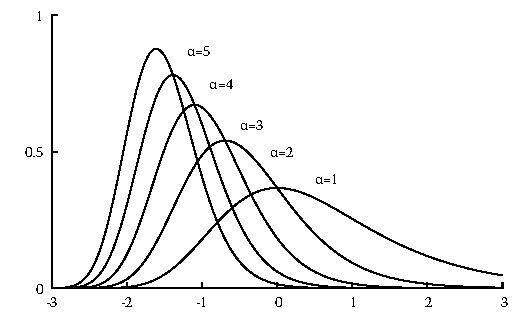
\includegraphics[width=\textwidth]{pdfGammaExp}   
\end{center}
\caption[Gamma exponential distributions]{Gamma exponential distributions, $\opr{GammaExp}(x\given 0,1,\alpha)$} 
\end{figure}


\begin{figure}[t]
\begin{center}
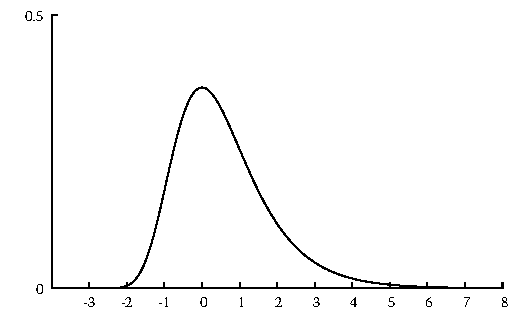
\includegraphics[width=\textwidth]{pdfGumbel}  
\end{center}
\caption[Gumbel distribution]{Standard Gumbel distribution, $\opr{StdGumbel}(x)$} 
\end{figure}


\begin{table}[tp]
\caption[Gamma-exponential distribution -- Special cases]{Special cases of the gamma-exponential family}
\begin{center}
{\renewcommand{\arraystretch}{1.25} 
\begin{tabular}{llcccl}
\eqref{GammaExp} &gamma-exponential &  $\nu$ & $\lambda$ & $\alpha$ 
\\ \hline
\eqref{StdGammaExp} & standard gamma-exponential &  $0$ & $1$ & $\alpha$  \\
\eqref{ChiSqrExp} & chi-square-exponential &$\ln 2 $ & $1$ & $\tfrac{k}{2}$ \\ 
\eqref{GenGumbel} &generalized Gumbel    & . & . & $n$ &  \\
\eqref{Gumbel} &Gumbel  &  . & . & 1 &  \\
\eqref{StdGumbel} &standard Gumbel &   0 & 1 & 1 & \\ 
\eqref{BHP} &BHP   & . & . & $\frac{\pi}{2}$ &  \\
\eqref{Moyal} & Moyal & . & . & \half 
%\\
% & \underline{Limits} \\
%\eqref{Normal} & normal  & . &  . & $\alpha$& $\lim_{\alpha\rightarrow\infty}$  \\
\end{tabular}
}
\end{center}
\end{table}


% !TEX encoding = UTF-8 Unicode 
% !TEX root = FieldGuide.tex

\begin{table*}[tp!]
\caption[Gamma-exponential distribution -- Properties]{Properties of the gamma-exponential distribution}
\begin{align*}
\text{\hyperref[PropertiesSec]{Properties}}  \quad& \\
\text{notation} \quad &  \op{GammaExp}(x \given \nu, \lambda, \alpha)  			\checked
\\
\text{PDF}\quad &   \frac{1}{ \Gamma(\alpha) |\lambda|}  \exp\Left\{- \alpha \Left(\frac{x-\nu}{\lambda}\Right) - \exp\Left(-\frac{x-\nu}{\lambda}\Right)  \Right\} \checked \hspace{-8em}												
\\
\text{CDF} \big/ \text{CCDF} \quad  &   Q\Left(\alpha, e^{-\frac{x-\nu}{\lambda} }\Right) 
& \lambda>0 \ \big/ \ \lambda<0  \checked
\\
\text{parameters}\quad &   \nu,\ \lambda,\ \alpha,\   \text{in } \Real, \ \alpha>0, \ 		\checked
\\
\text{support} \quad &   x \in [-\infty, +\infty]									\checked
\\
\text{mode} \quad  & \nu -\lambda \ln \alpha \checked
\\
\text{mean} \quad  &   \nu- \lambda \psi(\alpha)	\checked
\\
\text{variance} \quad  &  \lambda^2 \psi_1(\alpha)	\checked
\\
\text{skew} \quad  &   -\text{sgn}(\lambda) \tfrac{\psi_2(\alpha) }{  \psi_1(\alpha)^{3/2} }  \checked
\\
\text{ex. kurtosis} \quad  &     \tfrac{ \psi_3(\alpha) }{  \psi_1(\alpha)^{2}} \checked
\\
%\text{entropy} \quad  &  \ln \Gamma(\alpha) |\lambda|  - \alpha \psi(\alpha) + \alpha
%\\
\text{MGF} \quad  &   e^{\nu t } \frac{\Gamma(\alpha-\lambda t)}{\Gamma(\alpha)}  \checked
& \text{\cite{Johnson1995}}  %after Eq 22.227
\\
\text{CF} \quad  &  e^{i \nu t } \frac{\Gamma(\alpha-i \lambda t)}{\Gamma(\alpha)} \checked
% Johnson1995, Eq 22.211, modulo typos
\end{align*}
\end{table*}






\dist{Gumbel}  (Fisher-Tippett type I, Fisher-Tippett-Gumbel, Gumbel-Fisher-Tippett, FTG, log-Weibull, extreme value (type I),  doubly exponential, double exponential) distribution~\cite{Fisher1928,Gumbel1958, Johnson1995}:
\begin{align}
\label{Gumbel}
\opr{Gumbel}(x\given u,{\lambda}) 
&=
\frac{1}{|{\lambda}|}  \exp\left\{ -\left(\frac{x-u}{{\lambda}}\right) - \exp\left(-\frac{x-u}{{\lambda}}\right)  \right\} \checked
\\
&= \opr{GammaExp}(x\given u,{\lambda},1)  \checked
\notag
\end{align}
This is the asymptotic extreme value distribution for variables of ``exponential type'', unbounded with finite moments~\cite{Gumbel1958}.
With positive scale ${\lambda}>0$, this is an extreme value distribution of the maximum, with negative scale ${\lambda}<0$ an extreme value distribution of the minimum. Note that the Gumbel is sometimes defined with the negative of the scale used here.
% Mathematica uses negative scale. Wikipedia uses this scale.

The term ``double exponential distribution'' can refer to either Laplace or Gumbel distributions~\cite{Johnson1995}.


\dist{Standard Gumbel} (Gumbel) distribution~\cite{Gumbel1958}:
\begin{align}
\label{StdGumbel}
\opr{StdGumbel}(x) 
=&
  \exp\left\{- x - e^{-x} \right\}  \checked \\
=& \opr{GammaExp}(x\given 0,1,1)  \notag \checked
\end{align}
The Gumbel distribution with zero location and a unit scale.



\dist{BHP} (Bramwell-Holdsworth-Pinton) distribution~\cite{Bramwell1998, Bramwell2000}:
\begin{align}
\label{BHP}
\opr{BHP}(x\given \nu,\lambda) 
&=
\frac{1}{\Gamma(\tfrac{\pi}{2}) |\lambda|}  \exp\left\{ - \frac{\pi}{2}\left(\frac{x-\nu}{\lambda}\right) -  \exp\left(-\frac{x-\nu}{\lambda}\right)  \right\}  \checked
\notag
\\
&= \opr{GammaExp}(x\given \nu,\lambda,\frac{\pi}{2})   \checked
\end{align}
Proposed as a model of rare fluctuations in turbulence and other correlated systems.
% v0.6 flipped sign on lambda.


\dist{Moyal} distribution~\cite{Moyal1955}:
\begin{align}
\label{Moyal}
\opr{Moyal}(x\given \mu, \lambda) & = 
%\frac{1}{\sqrt{2\pi} }  \exp\left\{- \half x - \half  e^{-x}  \right\} 	\checked
%\\
\frac{1}{\sqrt{2\pi}  |\lambda|}  \exp\left\{- \half \left(\frac{x-\mu}{\lambda}\right) - \half \exp\left(- \frac{x-\mu}{\lambda}\right)  \right\} \checked
\\
&= \opr{GammaExp}(x\given \mu+ \lambda \ln 2, \lambda ,\half)  \checked
\notag
\end{align}
Introduced as analytic approximation to the  Landau distribution \eqref{Landau} \cite{Moyal1955}.



\SSec{Interrelations}

The name ``log-gamma'' arises because the standard log-gamma distribution is the logarithmic transform of the standard gamma distribution
\begin{align*}
\opr{StdGammaExp}(\alpha)  &\sim - \ln\Bigl( \opr{StdGamma}(\alpha) \Bigr) \checked
\\
\opr{GammaExp}(\nu, \lambda, \alpha)  &\sim -\ln\Bigl( \opr{Amoroso}(0, e^{-\nu},\alpha, \tfrac{1}{\lambda}) \Bigr) \checked
\end{align*}

The difference of two gamma-exponential distribution (with common scale) is a beta-logistic distribution \eqref{BetaLogistic}~\cite{Johnson1995}. % eq 22.212
\[
\opr{BetaLogistic}(x\given \pLoc_1-\pLoc_2,\pScale,\alpha,\gamma)   
& \sim \opr{GammaExp}_1(x\given \pLoc_1,\pScale,\alpha)  \notag \\ & \qquad -\opr{GammaExp}_2(x\given \pLoc_2,\pScale,\gamma)
\checked
\notag
\]
It follows that the difference of two Gumbel distributions \eqref{Gumbel} is a logistic distribution \eqref{Logistic}.

The gamma-exponential distribution is a limit of the Amoroso distribution \eqref{Amoroso}, and itself contains the normal \eqref{Normal} distribution as a limiting case.
\[
\lim_{\alpha\rightarrow\infty} \opr{GammaExp}(x\given  \mu+\sigma\sqrt{\alpha}\ln\alpha, \sigma\sqrt{\alpha},\alpha)
= \opr{Normal}(x\given \mu, \sigma)
\notag
\]


